\documentclass{article}
\usepackage{arxiv}

\usepackage[utf8]{inputenc}
\usepackage[english, russian]{babel}
\usepackage[T1]{fontenc}
\usepackage{url}
\usepackage{booktabs}
\usepackage{amsfonts}
\usepackage{nicefrac}
\usepackage{microtype}
\usepackage{lipsum}
\usepackage{graphicx}
\usepackage{natbib}
\usepackage{doi}
\newcommand*{\defeq}{\stackrel{\mathsmaller{\mathsf{def}}}{=}}




\title{Compression for Federated Random Reshuffling}

\author{ Tikhon Antyshev\\
	MIPT\\
	\And
	Grigory Malinovsky \\
	KAUST\\
	%% \AND
	%% Coauthor \\
	%% Affiliation \\
	%% Address \\
	%% \texttt{email} \\
	%% \And
	%% Coauthor \\
	%% Affiliation \\
	%% Address \\
	%% \texttt{email} \\
	%% \And
	%% Coauthor \\
	%% Affiliation \\
	%% Address \\
	%% \texttt{email} \\
}
\date{}

\renewcommand{\shorttitle}{\textit{arXiv} Template}

%%% Add PDF metadata to help others organize their library
%%% Once the PDF is generated, you can check the metadata with
%%% $ pdfinfo template.pdf
\hypersetup{
pdftitle={A template for the arrxiv style},
pdfsubject={q-bio.NC, q-bio.QM},
pdfauthor={David S.~Hippocampus, Elias D.~Striatum},
pdfkeywords={First keyword, Second keyword, More},
}

\begin{document}
\maketitle

\begin{abstract}
	Federated Random Reshuffling (FedRR) is a recently developed method for federated training of supervised machine learning models via empirical risk minimization. It utilizes Random Reshuffling (RR), a variant of Stochastic Gradient Descent (SGD)along with Local Training carried out by the clients. We propose integration of compression techniques in FedRR, reducing the number of communicated bits in order to overcome communication bottleneck, furthermore we integrate server-side optimization (Server Stepsizes) to get improvement in theory and practice. To the best of our knowledge, this is the first time FedRR will be combined with Server Stepsizes and Compressed Iterates at the same time. 

\end{abstract}


\keywords{Machine Learning \and Federated Learning \and Random Reshuffling }

\section{Introduction}
%\lipsum[2]
%\lipsum[3]
Modern machine learning models heavily rely on Empirical Risk Minimization for supervised training training. The  success of this approach itself can be attributed to a plentiful amount of data available.

\subsection{Problem Statement}
We consider the standard finite-sum optimization formulation of
federated learning problem:
\[
    x_* = \arg\min_{x \in \mathbb{R}^d}\big[f(x) \defeq \frac{1}{M}\sum_{m=1}^M f_m(x) \big]
\]
\[f_m(x) \defeq \frac{1}{n}\sum_{i = 1}^n f_m^i(x)\]
Where M is number of clients in current task, $f_m:\mathbb{R}^d \rightarrow \mathbb{R}$ is the loss of the model $x$ on the training data subset owned by client or device $m$, which has the finite-sum structure, comprised of $f_m^i: \mathbb{R}^d \rightarrow \mathbb{R}$ - loss of model $x$ on training point $i \in \overline{1, n}$. We shall also assume that $ \forall \; m,\, i:\: f_m^i$ is differentiable and consider strongly convex, convex and non-convex modes.

\subsection{}

\section{Contributions}
\label{sec:headings}

%\lipsum[4] See Section \ref{sec:headings}.

%\subsection{Headings: second level}
%\lipsum[5]
%\begin{equation}
%	\xi _{ij}(t)=P(x_{t}=i,x_{t+1}=j|y,v,w;\theta)= {\frac {\alpha _{i}(t)a^{w_t}_{ij}\beta _{j}(t+1)b^{v_{t+1}}_{j}(y_{t+1})}{\sum _{i=1}^{N} \sum _{j=1}^{N} \alpha _{i}(t)a^{w_t}_{ij}\beta _{j}(t+1)b^{v_{t+1}}_{j}(y_{t+1})}}
%\end{equation}

%\subsubsection{Headings: third level}
%\lipsum[6]

%\paragraph{Paragraph}
%\lipsum[7]
\section{Preliminaries}


\section{Theory}

\section{Experiments}
The goal of the experiment is to demonstrate improvements of implementing Compressed Iterates with Server Step-Sizes method. We
run our experiment on $l2$-regularized logistic regression
with the ‘a1a’ dataset from LibSVM.
As a baseline solution we will be demonstrating the results of Proximal and Federated RR. Afterwards, we shall compare performance for proposed algorithm and versions that use either only Server Step-sizes or only Compressed Iterates.
\begin{figure}[h]
\begin{minipage}[h]{0.49\linewidth}
\center{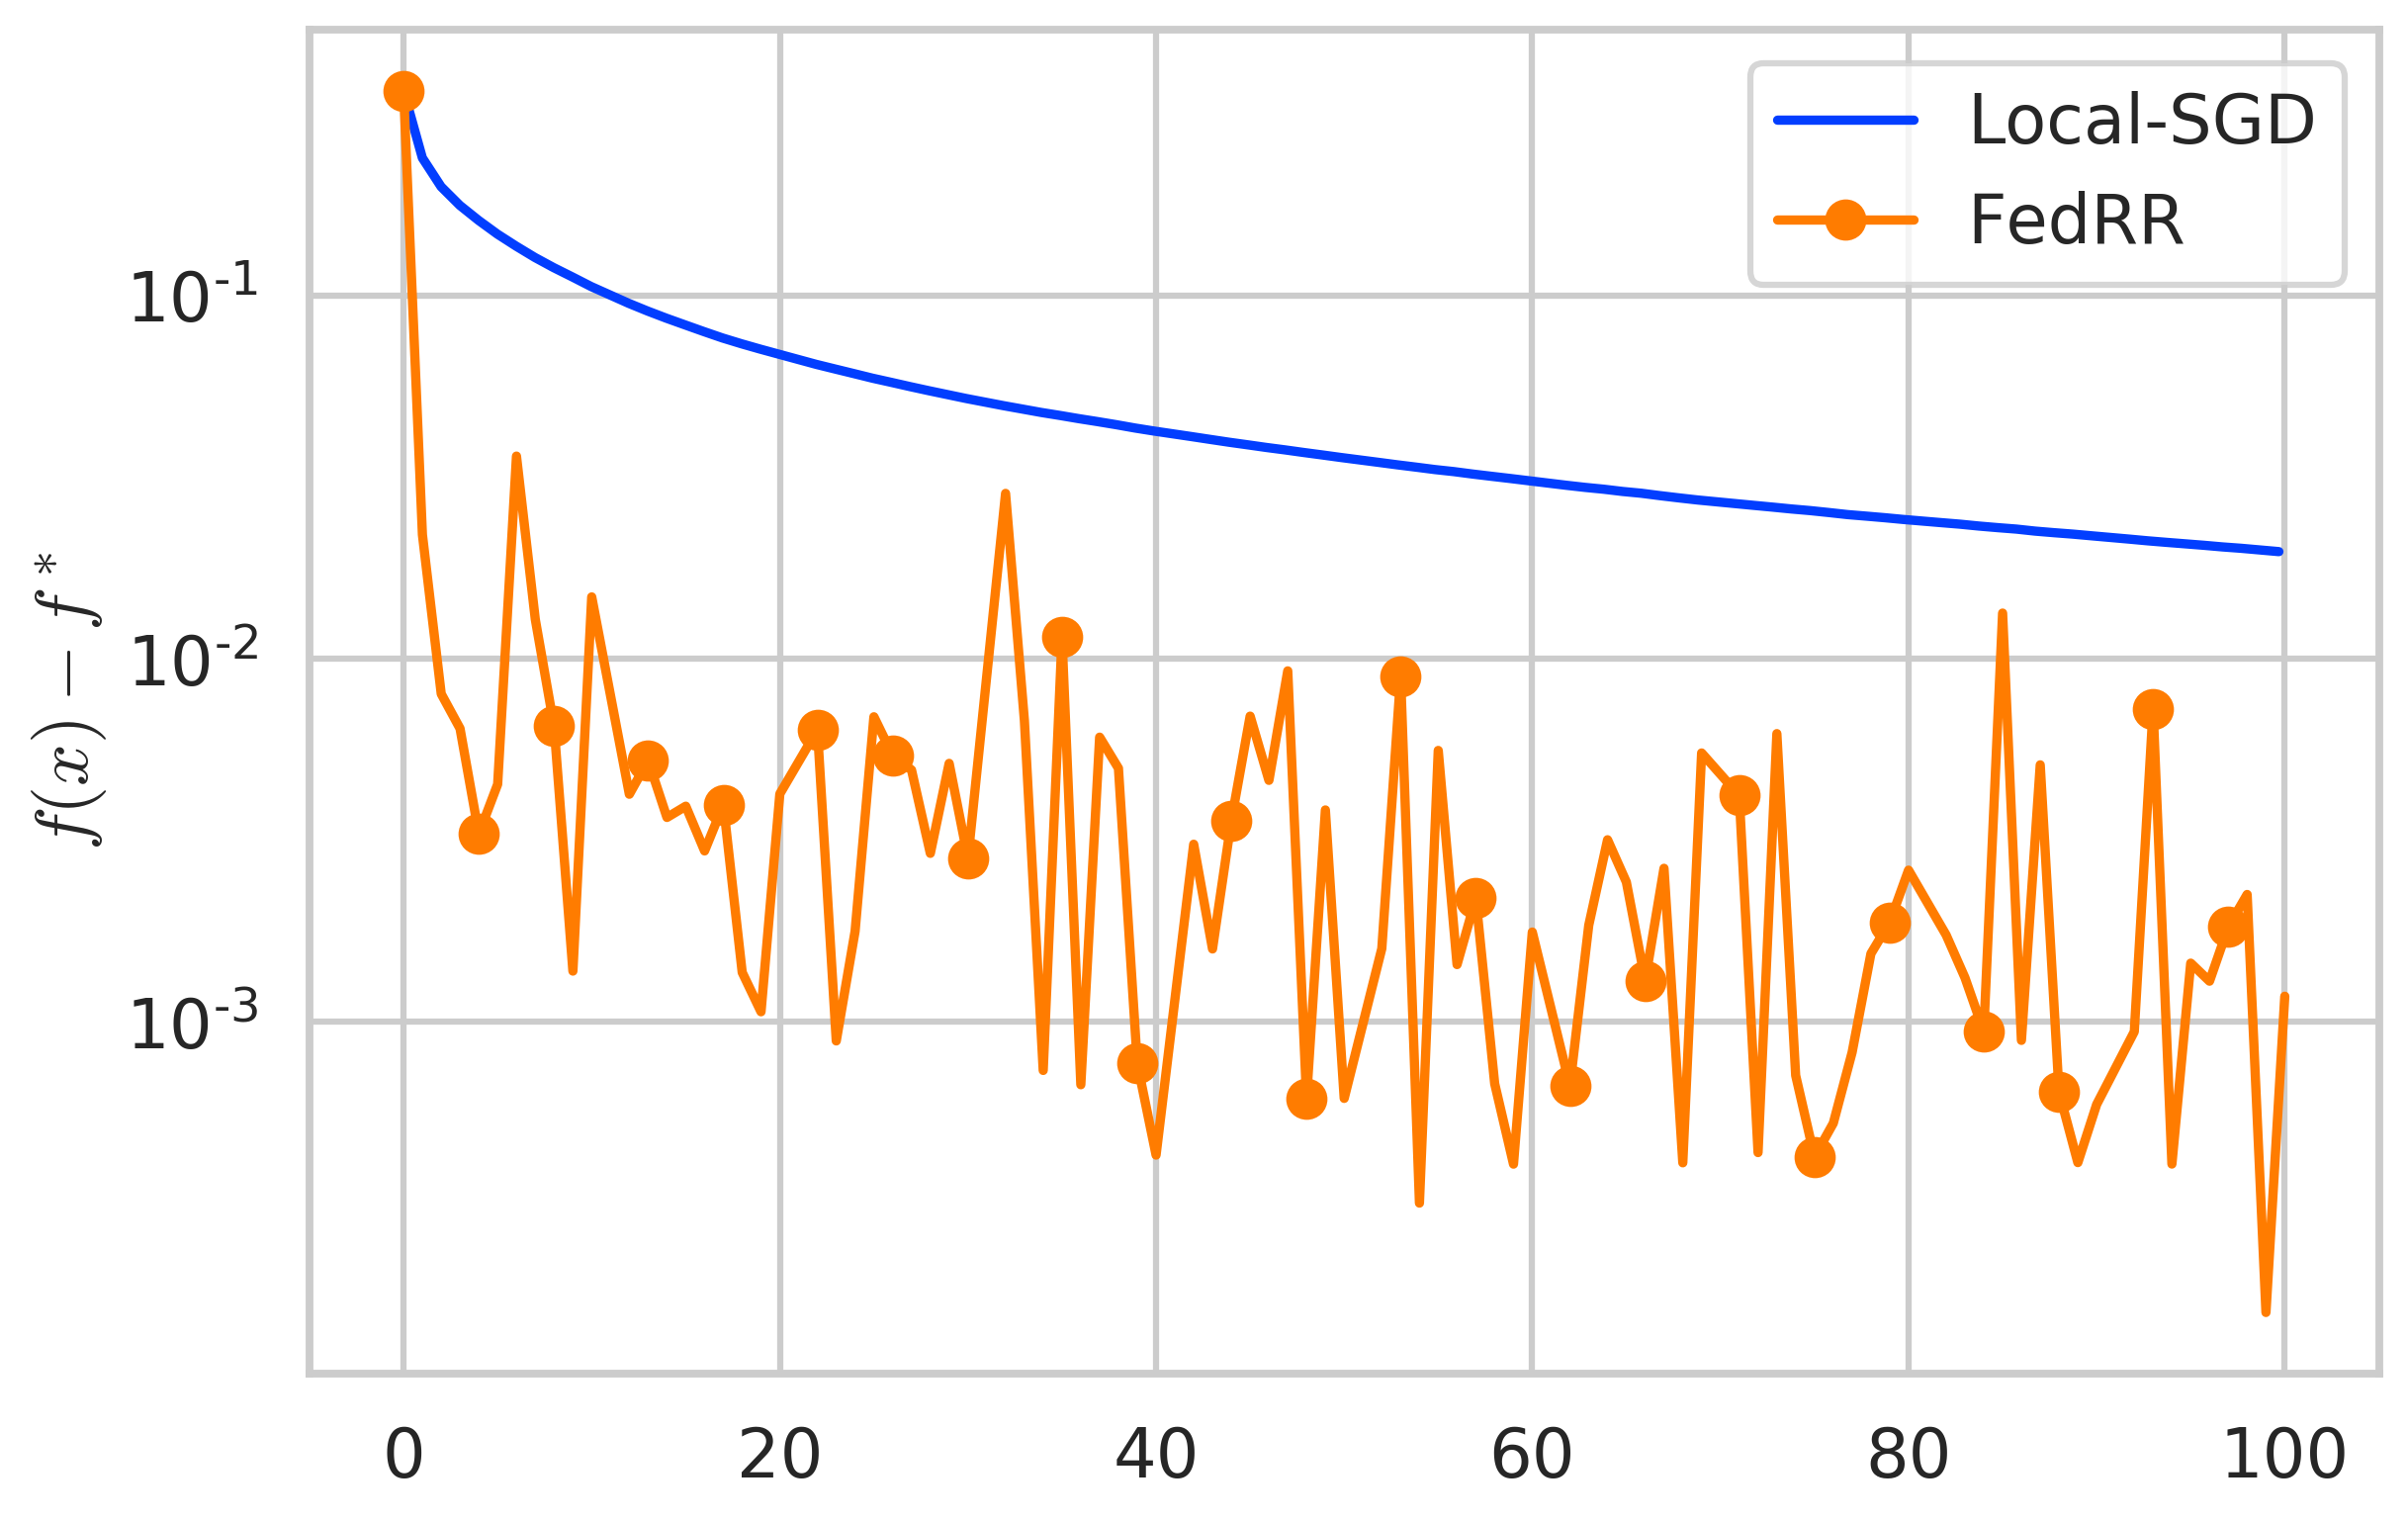
\includegraphics[scale=0.35]{figures/fedVSsgd_a1a.png} \\ Local SGD and Federated RR}
\end{minipage}
\hfill
\begin{minipage}[h]{0.49\linewidth}
\center{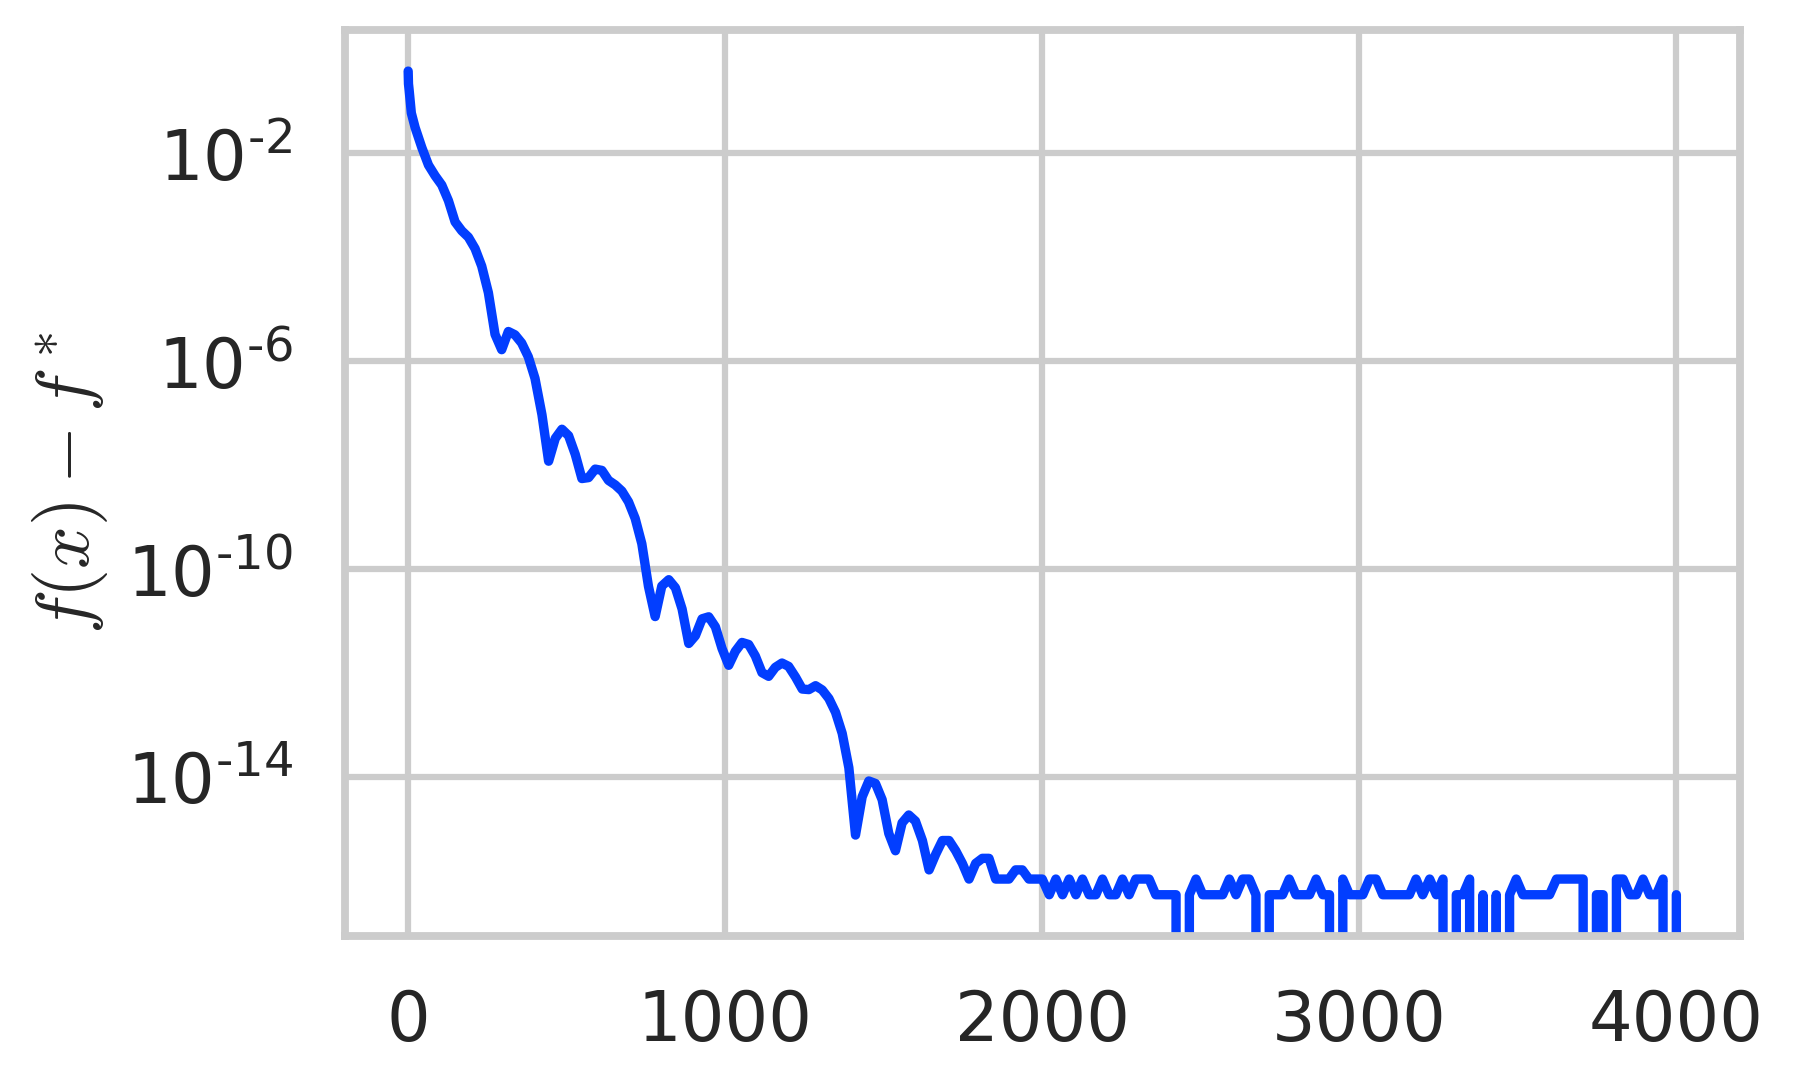
\includegraphics[scale=0.5]{figures/RestNest.png} \\ Performance of Nesterov method}
\end{minipage}
\end{figure}

%
%\begin{figure}[h]
%\begin{minipage}[h]{0.49\linewidth}
%\center{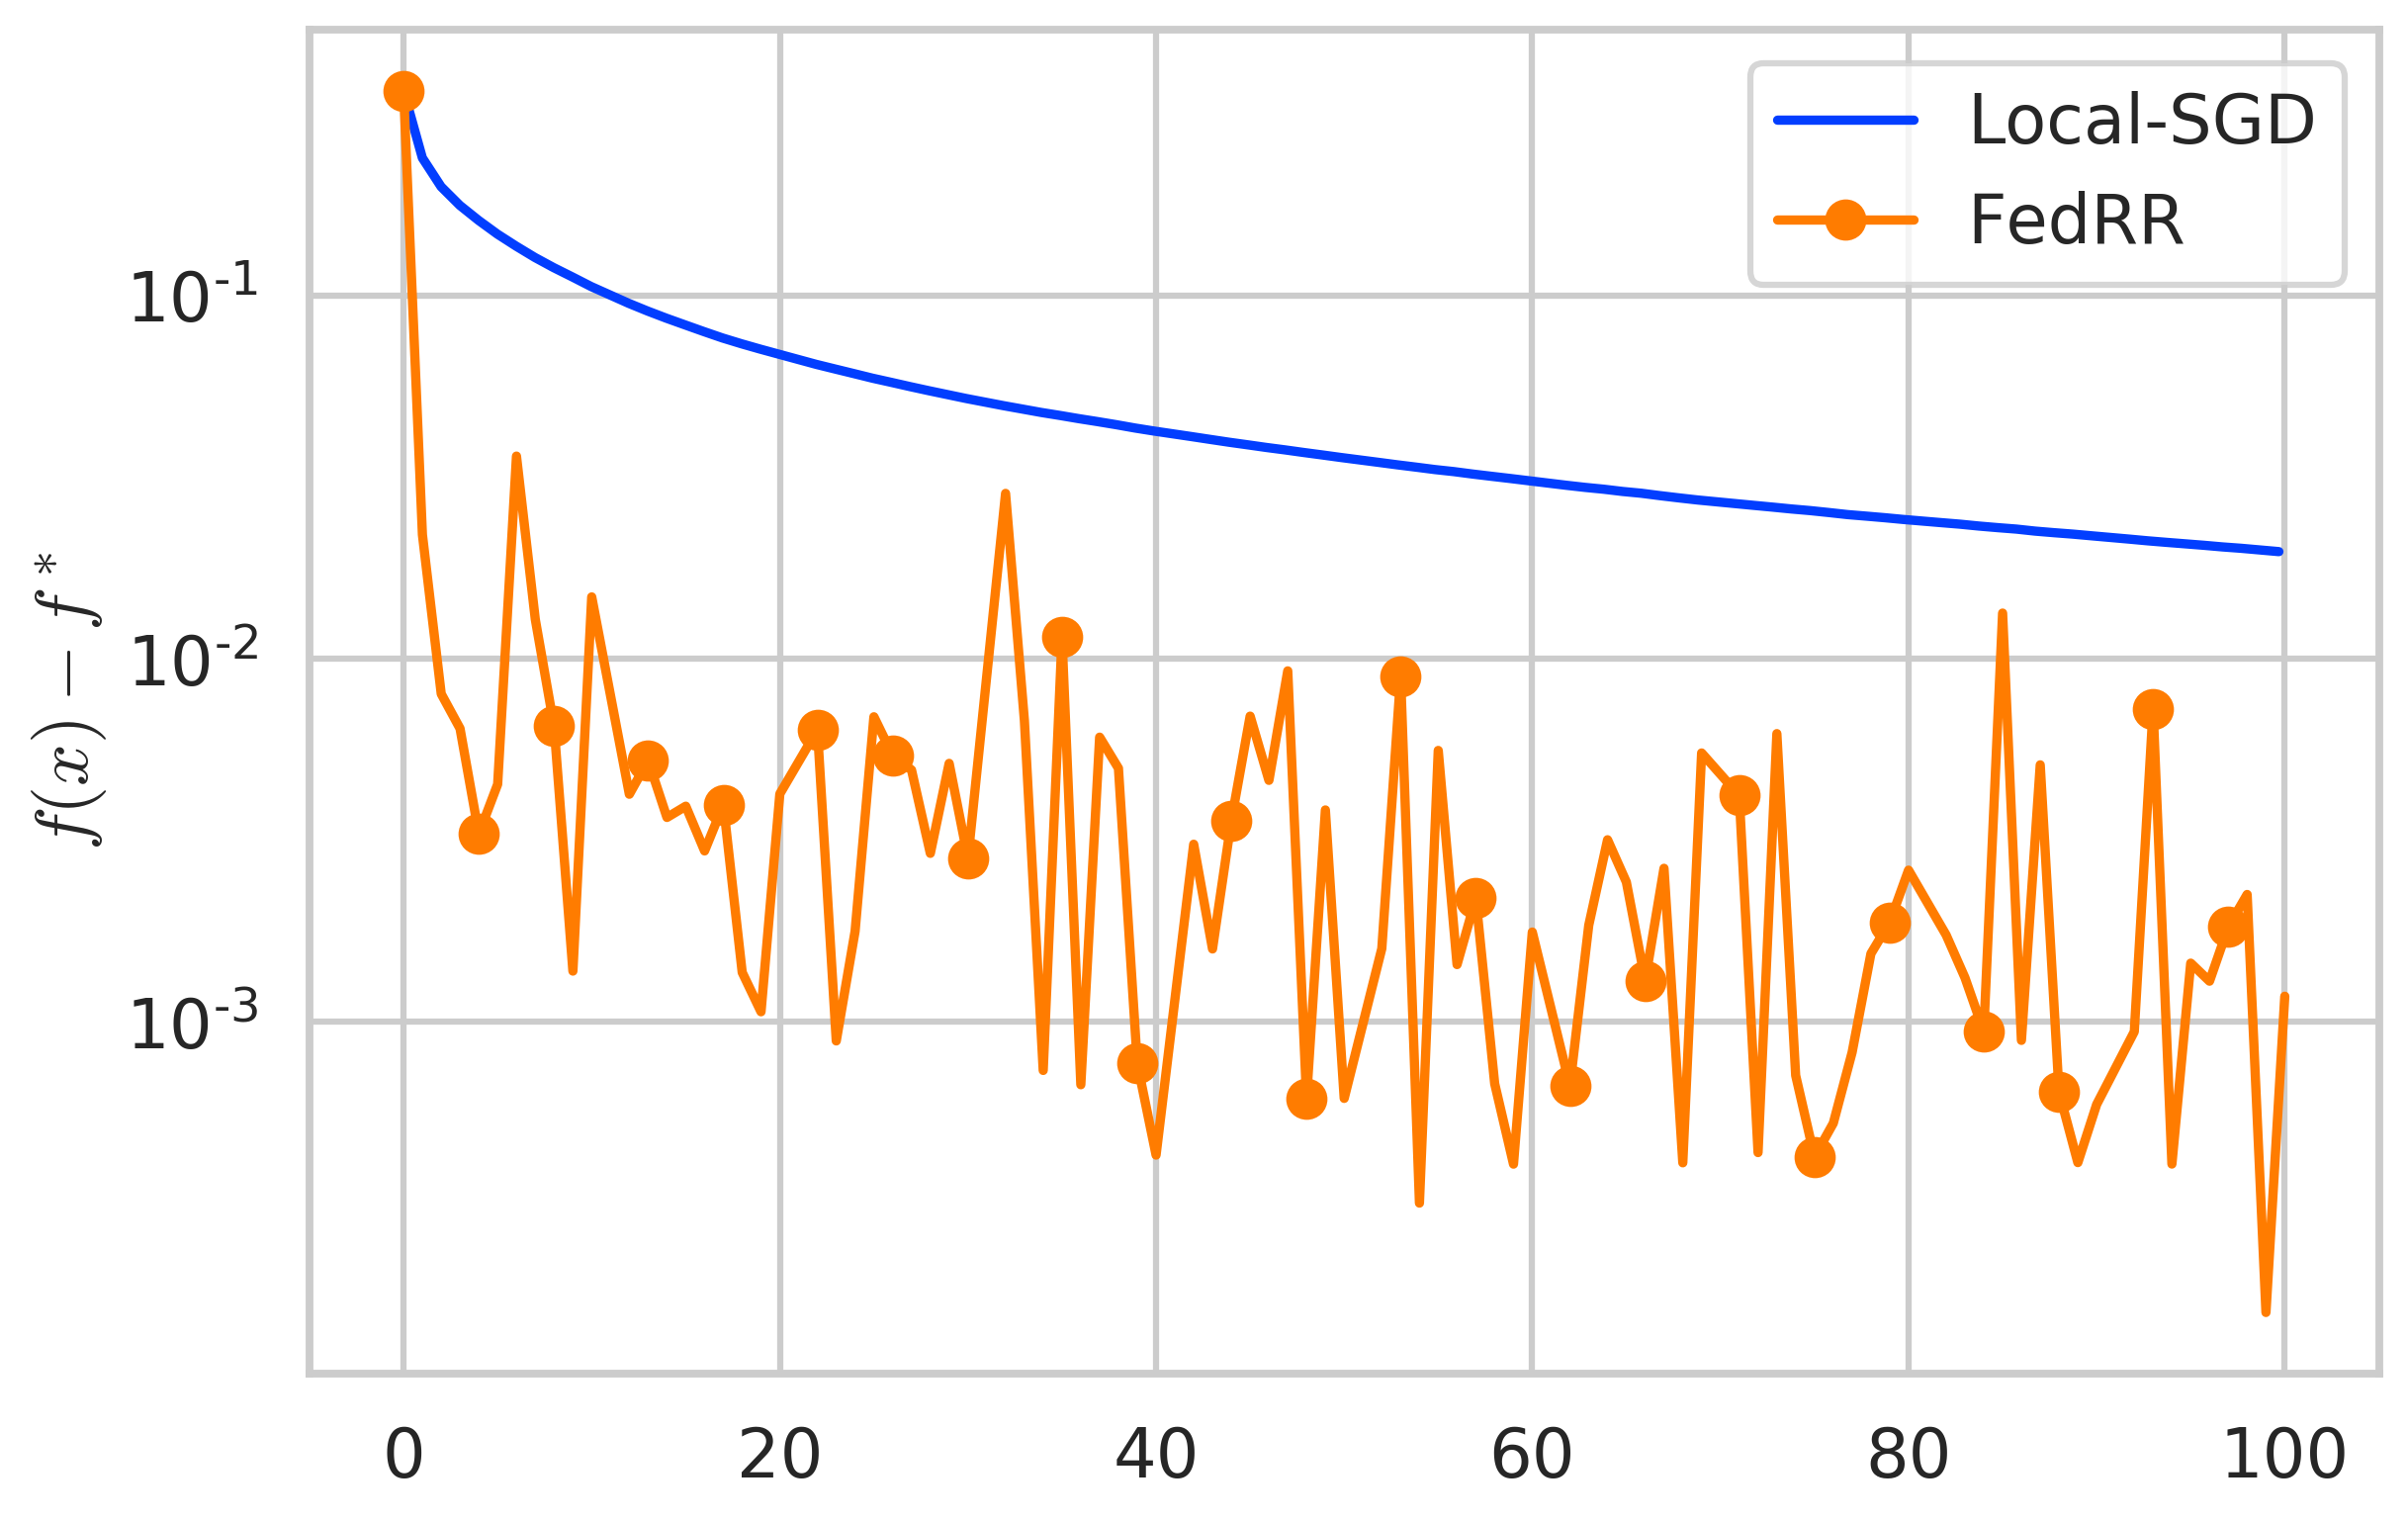
\includegraphics[scale=0.35]{figures/fedVSsgd_a1a.png} \\ Data %distribution before SMOTE}
%\end{minipage}
%\hfill
%\begin{minipage}[h]{0.49\linewidth}
%\center{\includegraphics[scale=0.35]{synth_data_after_smote.png} \\ %%Data distribution after SMOTE}
%\end{minipage}
%\end{figure}


\section{Examples of citations, figures, tables, references}
%\label{sec:others}

\subsection{Citations}
%Citations use \verb+natbib+. The documentation may be found at
%\begin{center}
	%\url{http://mirrors.ctan.org/macros/latex/contrib/natbib/natnotes.pdf}
%\end{center}

%Here is an example usage of the two main commands (\verb+citet+ and %\verb+citep+): Some people thought a thing \citep{kour2014real, hadash2018estimate} but other people thought something else \citep{kour2014fast}. Many people have speculated that if we knew exactly why \citet{kour2014fast} thought this\dots

\subsection{Figures}
%\lipsum[10]
%See Figure \ref{fig:fig1}. Here is how you add footnotes. \footnote{Sample of the first footnote.}
%\lipsum[11]

%\begin{figure}
%	\centering
%	\includegraphics[width=0.5\textwidth]{../figures/log_reg_cs_exp.eps}
%	\caption{Sample figure caption.}
%	\label{fig:fig1}
%\end{figure}

\subsection{Tables}
%See awesome Table~\ref{tab:table}.

%The documentation for \verb+booktabs+ (`Publication quality tables in LaTeX') is available from:
%\begin{center}
%	\url{https://www.ctan.org/pkg/booktabs}
%\end{center}


%\begin{table}
%	\caption{Sample table title}
%	\centering
%	\begin{tabular}{lll}
%		\toprule
%		\multicolumn{2}{c}{Part}                   \\
%		\cmidrule(r){1-2}
%		Name     & Description     & Size ($\mu$m) \\
%		\midrule
%		Dendrite & Input terminal  & $\sim$100     \\
%		Axon     & Output terminal & $\sim$10      \\
%		Soma     & Cell body       & up to $10^6$  \\
%		\bottomrule
%	\end{tabular}
%	\label{tab:table}
%\end{table}

\subsection{Lists}
%\begin{itemize}
	%\item Lorem psum dolor sit amet
	%\item consectetur adipiscing elit.
	%\item Aliquam dignissim blandit est, in dictum tortor gravida eget. In ac %rutrum magna.
%\end{itemize}


\bibliographystyle{unsrtnat}
\bibliography{references}

\end{document}

\end{document}
